\section{El teorema de la proyección ortogonal}
\begin{teo} \label{Teo:proyOrt}
\TODO{cambiar notación.}
(\textbf{de la proyección ortogonal}
~\cite{Nimark}):
Sean $H$ un espacio de Hilbert, $W$ un subespacio cerrado de $H$. 
Para todo $x \in H$ existe un único $\hat{x} \in W $ tal que
\[
||x- \hat{x}|| = inf_{y \in W}|| x-y ||;
\]
además, $\hat{x}$ es el único elemento de $W$
tal que $x-\hat{x} \in W^{\perp} $.
\end{teo}


En general, si $H$ es un espacio métrico y W es un subconjunto
de este, puede definirse la distancia de un punto $x \in H$ a W como
el ínfimo del conjunto de distancias entre $x$ y puntos de $W$:

\[
d(x,W)=inf\{||x-y||: y \in W \}.
\]
\noindent 
Tal ínfimo existe por estar el conjunto descrito acotado inferiormente,
por ejemplo, por el cero. El teorema de la proyección 
\ref{Teo:proyOrt} nos dice entonces que,
en el contexto de espacios de Hilbert, si $W$ es un subespacio de $H$
que además es cerrado \footnote{Cuidado aquí: hay dos nociones distintas de 
cerradura involucradas. Como el espacio métrico $H$ es un espacio vectorial
normado, con ``subespacio'' nos referimos a un subespacio vectorial de $H$,
no a un mero subconjunto de este; es decir, requerimos que $W$ sea cerrado bajo
las operaciones de espacio vectorial. Se pide además que $W$ (pensado
como subconjunto del espacio métrico $H$) sea cerrado, es decir, que contenga
a todos sus puntos límite
(c.f. definición \TODO{Munkres}).}, tal ínfimo se alcanza, es decir, existe un punto
(además, único) $\hat{x}$ de $W$ que minimiza la distancia a $x$. \\

En este trabajo, 
el espacio con producto punto
particular que nos concierne 
es $\IR^{n}$ con el producto punto usual; por ser
este un espacio finito-dimensional, 
cualquier subespacio de este es cerrado
(~\cite{Kreyszig}, Thm. 2.4-3),
luego, el teorema de la proyección siempre aplica. 

En general, si $W$ es un subespacio cerrado de
un espacio de Hilbert $H$, gracias a la unicidad
establecida en el teorema \ref{Teo:proyOrt},
podemos definir la función \textbf{proyección a $W$}
como sigue:

\begin{equation}
\label{eq3: 1Dic}
\aplica{\Pi_{W}}{H}{W}{x}{\hat{x}},
\end{equation}
donde $\hat{x}$ es el único vector del que se habla
en el teorema \ref{Teo:proyOrt}.


Puede pensarse a esta como la función que a cada elemento
$x$ del espacio le asocia ``su representante'' del espacio $W$
más cercano. Otra consecuencia de la unicidad establecida en el teorema
\ref{Teo:proyOrt} es la linealidad de la función
$\Pi_{W}$. 

\begin{cor}
Sean $V$ es un espacio de Hilbert, $W$ un subespacio cerrado de 
$V$ cuyo complemento ortogonal también es cerrado en $V$ 
\footnote{De hecho, una vez establecida la continuidad
del producto punto más adelante en la
proposición \ref{prop: continuidad del producto punto}, podremos
quitar la hipótesis de que $W^{\perp}$ sea cerrado, pues esto
será consecuencia de que $W$ lo sea (si $(a_{n})_{n \in \IN}$
es una sucesión en $W^{\perp}$ convergente a algún $a \in V$,
entonces, para todo $w \in W$,
$\langle a, w \rangle = 
\langle \limite{n \rightarrow \infty}{a_{n}}, w \rangle
= \limite{n \rightarrow \infty}{\langle a_{n},w \rangle}=
\limite{n \rightarrow \infty}{0}=0$,
luego, $a \in W^{\perp}$ ).}. Entonces,
\begin{itemize}
\item Para todo $v \in V$, $v= \Pi_{W}(v)+ \Pi_{W^{\perp}}(v)$.
\item $\Pi_{W}: V \longrightarrow Z$ es un operador autoadjunto.
\end{itemize}
\end{cor}
\noindent
\textbf{Demostración.}
Sea $v \in V$ cualquiera; según el teorema
de la proyección
\ref{Teo:proyOrt}, 
\begin{equation}
\label{eq3: 1En}
v - \Pi_{W}(v) \in W^{\perp};
\end{equation}
además,
\begin{equation}
\label{eq4: 1En}
v-(v-\Pi_{W}(v))= \Pi_{W}(v) \in W \subseteq (W^{\perp})^{\perp};
\end{equation}
puesto que, según el teorema de la proyección, 
$\Pi_{W^{\perp}}(v)$ se caracteriza por ser el 
único elemento de $W^{\perp}$ tal que 
$v-\Pi_{W^{\perp}}(v) \in (W^{\perp})^{\perp}$,
concluimos por \eqref{eq3: 1En} y \eqref{eq4: 1En}
la igualdad
\[
v-\Pi_{W}(v)= \Pi_{W^{\perp}}(v).
\]
Esto demuestra el primer punto del corolario. Para demostrar
el segundo, o sea, que para cualesquiera
$u, v \in V$ se tiene que
\[
\langle u, \Pi_{W}(v) \rangle = 
\langle \Pi_{W}(u), v \rangle,
\]
sólo observe que,
usando el primer punto ya demostrado, tenemos que
\begin{align*}
\langle u, \Pi_{W}(v) \rangle = & 
\langle \Pi_{W}(u) + \Pi_{W^{\perp}}(u), \Pi_{W}(v) \rangle  \\
= & \langle \Pi_{W}(u), \Pi_{W}(v) \rangle  + 
\langle \Pi_{W^{\perp}}(u), \Pi_{W}(v) \rangle  \\
= & \langle \Pi_{W}(u), \Pi_{W}(v) \rangle  ,
\end{align*}
donde la última igualdad se da porque $\Pi_{W}(v) \in W$ y 
$\Pi_{W^{\perp}}(v) \in W^{\perp}$ (luego,
son vectores mutuamente perpendiculares), y, análogamente,
\[
\langle \Pi_{W}(u), v \rangle  =  
\langle \Pi_{W}(u), \Pi_{W}(v)\rangle .
\]
\QEDB
\vspace{0.2cm}


\noindent Ya que estamos hablando de proyecciones ortogonales,
usemos estas para ddemostrar
una de las desigualdades
más importantes con las que se cuenta en un espacio
con producto punto.

\begin{teo}
(\textbf{Desigualdad de Cauchy-Schwarz}) \label{Teo:CauchySchwarz}
Sea $V$ un $\IR-$espacio vectorial con producto punto 
$ \langle \cdot  , \cdot  \rangle$.
\begin{equation}
\label{eq0: 12Feb}
\forall v , w \in V : \hspace{0.5cm}
|\langle  v , w \rangle | \leq ||v|| \cdot ||w||,
\end{equation}
siendo $|| \cdot ||$
la norma inducida por el producto punto.
\TODO{Además, la igualdad en \eqref{eq0: 12Feb} se da
sí y sólo si $v$ es múltiplo escalar de $w$.}
\end{teo}
\noindent
\textbf{Demostración.}
(basada en la demostración
ofrecida en ~\cite{Lang}, p. 292)
\begin{itemize}
\item Si alguno de los vectores $v$ o $w$ es cero,
la igualdad se da trivialmente (el vector cero tiene norma
cero y es ortogonal a cualquier vector). 

\item Si $v=a w$ para algun real $a$, también se 
da la igualdad:
\[
|\langle  v , w \rangle | =
|\langle  aw , w \rangle | = |a| \cdot  |\langle  w , w \rangle | =  
 |a| \cdot ||w||^{2}
=||aw|| \cdot ||w|| = ||v|| \cdot ||w||.
\]
\item Supongamos por último que no ocurre ninguno
de los casos de los puntos anteriores, o sea, que
$v$ y $w$ son linealmente independientes. \\
Si $c:=\frac{\langle v , w \rangle}{\langle w , w \rangle}$,
según G-S (\ref{Teo:Gram-Schmidt}), 
$v-cv$ y $cw$ son vectores ortogonales cuya suma es $v$;
así, por el teorema de pitágoras,
\begin{align*}
||v||^{2} & = ||v-cw||^{2} + ||cw||^{2} \\
& \geq ||cw||^{2}= |c|^{2} \cdot ||w||^{2} \\
& = \frac{\langle v , w \rangle ^{2}}{||w||^{4}}||w||^{2}
= \frac{\langle v , w \rangle ^{2}}{||w||^{2}},
\end{align*}
luego, 
\[
\langle  v , w \rangle ^{2}  \leq ||v||^{2} \cdot ||w||^{2}.
\]
Tomando raíces cuadradas en ambos lados de la
desigualdad llegamos a la desigualdad deseada. \QEDB
\end{itemize}
\vspace{0.2cm}


Esta desigualdad, que relaciona la norma de los
vectores cuyo producto punto se calcula, permite
establecer la continuidad del producto punto. \\


\begin{prop} \label{prop: continuidad del producto punto}
La función $\langle  \cdot , \cdot \rangle :
V \times V \longrightarrow \IR $ es continua.
\end{prop}
\noindent
\textbf{Demostración.}
\TODO{mejor pon esta introducción afuera, mucho más arriba:
Hay que aclarar que $V$ tiene estructura
de espacio métrico, siendo la métrica inducida por
la norma $|| \cdot || $(que, a su vez, fue inducida
por el producto punto $\langle  \cdot , \cdot$ )
dada por la relación }

\[
d(v,w)= ||v-w||, \hspace{1cm} v, w \in V.
\]
Dotamos al producto cartesiano $V \times V $
estructura de espacio métrico al \TODO{...} \\


Demostrar la continuidad de 
$\langle  \cdot , \cdot \rangle$ significa entonces
probar que
\[
(x_{n}, y_{n}) \rightarrow (x,y) \hspace{0.5cm}
\Rightarrow \hspace{0.5cm} \limite{n \rightarrow \infty}{
\langle  x_{n} , y_{n} \rangle} = \langle  x , y \rangle .
\]
Hagamos esto. Puesto que
\[
x_{n} \rightarrow x \hspace{0.4cm} \text{y}
\hspace{0.4cm} y_{n} \rightarrow y, 
\]

\noindent
los módulos de los vectores $x_{n}$ y $y_{n}$ 
están acotados, digamos por las constantes $K$ y $M$. \\
Por la bilinealidad del producto punto, para toda $n$
\[
\langle x_{n}-x , y_{n}-y \rangle =
\langle x_{n}, y_{n}\rangle -
\langle x_{n} , y \rangle -
\langle x , y_{n} \rangle +
\langle x , y \rangle ,
\]
\noindent
luego, por la desigualdad triangular y la de Cauchy-Schwarz
(\ref{Teo:CauchySchwarz}),
\begin{align*}
0 & \leq |\langle x_{n}, y_{n}\rangle - \langle x , y \rangle|
& \leq & |\langle x_{n}-x , y_{n}-y \rangle| +
|\langle x_{n} , y \rangle| + |\langle x , y_{n} \rangle| \\
&& \leq & ||x_{n}-x|| \cdot ||y_{n}-y|| + ||x_{n}||\cdot ||y_{n}||
+||x|| \cdot ||y_{n}|| \\
&& \leq & ||x_{n}-x|| \cdot ||y_{n}-y|| + K\cdot ||y_{n}||
+M \cdot ||x||; 
\end{align*}
Como $x_{n} \rightarrow x$ y $y_{n} \rightarrow y$,
el lado derecho de la desigualdad tiende a cero
conforme $n \rightarrow \infty$. Por el teorema de la compresión,
concluimos que
\[
\limite{n \rightarrow \infty}{|\langle x_{n}, y_{n}\rangle - \langle x , y \rangle|}=0,
\]
o sea, que 
$ \limite{n \rightarrow \infty}{
\langle  x_{n} , y_{n} \rangle} = \langle  x , y \rangle$.
\QEDB
\vspace{0.2cm}


\begin{comment} Esto es algo que hice que, ahora sé, es incorrecto. \\ 
Una vez introducidas las proyecciones ortogonales, podemos
establecer la equivalencia entre nuestra definición de base ortonormal
de un espacio con producto punto y la dada en \TODO{Kolmogorov [--]}
(que corresponde al segundo punto del siguiente teorema);
esto nos interesa porque, en el desarrollo del trabajo, muchas
veces usaremos el punto de vista dado por este último.

\begin{teo}
Sean $V$ un espacio con producto punto $< , >$, $B=\{ x_{\alpha} \}_{\alpha \in \Delta}$
un subconjunto ortonormal de $V$. 
\TODO{de hecho, nunca usas la ortonormalidad.}
Las siguientes
proposiciones son equivalentes:
\begin{enumerate}
\item $B$ es BON de $V$ (o sea, todo elemento de $V$ puede
expresarse de forma única como combinación lineal finita de elementos de $B$,
i.e. $span(B)=V$)
\item El subespacio cerrado de $V$ más pequeño que contiene a $B$
es él mismo, o sea,
\[
 \overline{B}= V,
\]
es decir, $B$ es denso en $V$ (\TODO{definición
válida en cualquier espacio topológico. Introduce antes la definición
general y la caracterización en términos de sucesiones de la cerradura
de un subconjunto cualquiera válida
en espacios métricos.}). \footnote{\TODO{en este caso se
dice que el sistema $B$ es completo, verdad?}}
\item $ \overline{span}(B)=V$.
\end{enumerate}
\end{teo}
\begin{dem}
Demostremos las equivalencias
\[
1) \Longleftrightarrow 3) \hspace{0.3cm} \text{y} \hspace{0.3cm}
3) \Longleftrightarrow 2). 
\]

\TODO{ya no estoy segura entre la equivalencia de 1 con 3. Recuerda
que el profesor te dijo que, en el caso inifinito dimensional, importan
más los subconjuntos densos a las bases del espacio (que siempre existen).
De todas formas, como usas el nombre ``base'', deberías aclarar
esto en la teoría.}

\begin{itemize}
\item[ $1) \Rightarrow  3)$] Sea $v \in V$; como
$B$ es base de este espacio, $v \in span(B)$, luego, 
$v$ es trivialmente elemento de la cerradura de $span(B)$.

\item[$3) \Rightarrow  1)$] Supongamos, por el contrario, que
$span(B) \subsetneq V $; sea pues $v \in V - span(B)$.
\TODO{no sé si aquí hay un error en el argumento; ¿cómo
estoy segura de que tal proyección existe? recuerda que el teorema
de la proyección ortogonal habla en términos de subespacios
CERRADOS.}
Sea $v':= \Pi_{span(B)}(v)$; puesto que $v'$ es elemento de 
$span(B)$ y $v$ no, estos son vectores distintos entre sí, luego,
\[
\epsilon := ||v-v'|| >0.
\]
Ahora bien, para este $\epsilon$, 
como span(B) es denso en $V$, existe $v'' \in span(B)$ tal que
\[
|| v-v'' || < \frac{\epsilon}{2};
\]
esto contradice el que $v'$ sea el elemento de $span(B)$ más
cercano a $v$.

\item[ $3) \Rightarrow  2)$]
Si $W$ es un subespacio cerrado de $V$ que contiene a $B$,
entonces también contiene a su span, luego, contiene a su cerradura, o sea, 
\[
V= \overline{span}(B) \subseteq W,
\]
luego, $W=V$.

\item[ $2) \Rightarrow  3)$] Puesto que el que un conjunto esté
contenido en otro implica que la cerradura del primero esté contenida
en la cerradura del segundo, tenemos que
\[
V = \overline{B} \subseteq \overline{span}(B) 
\subseteq \overline{V} =V. 
\]
\end{itemize}
\QEDB
\end{dem}
\end{comment}

\subsection{Ángulo entre elementos de un espacio con producto punto}

Es gracias a la desigualdad de Cauchy-Schwarz
que es posible introducir una de las nociones
más valiosas con las que se cuenta en un espacio
vectorial con producto punto, a saber, la de ángulo entre dos
vectores.

Si $v$ y $w$ son dos elementos no cero de $V$, entonces,
según el teorema \ref{Teo:CauchySchwarz},
\[
-1 \leq \frac{\langle v, w \rangle}{||v|| \cdot ||w||} \leq 1,
\]
luego, puesto que la función coseno es una biyección
del intervalo $[0, \pi]$ al intervalo $[-1,1]$,
tenemos que existe un único elemento 
$\theta \in [0, \pi]$ tal que

\[
cos(\theta)= \frac{\langle v, w \rangle}{||v|| \cdot ||w||};
\]
a tal número $\theta$ se le denomina el 
\textbf{ángulo formado por los vectores $v$ y $w$}.

\begin{marginfigure}
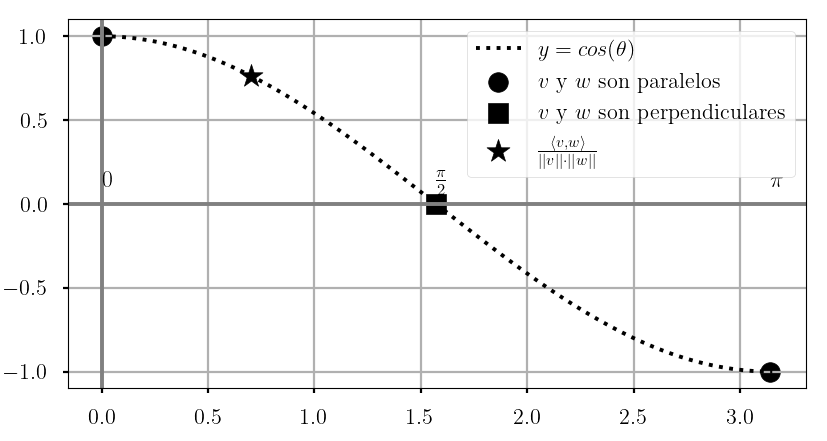
\includegraphics[scale=0.1]{coseno}
\end{marginfigure}

Si alguno de estos dos vectores fuese cero, definimos
el ángulo entre estos como cero. \TODO{Aquí deberías
de poner qué significan los casos extremos. Recuerda
la teoría de Spivak, cálculo en varias variables.}








